\section{COMPARATIVA CON OTROS COMPONENTES}

La elección de \emph{Arduino Yún} se ha realizado teniendo en cuenta las alternativas existentes en el mercado, encontrando que es la más adecuada para el tipo de proyecto que se va a realizar. A continuación se muestran algunos de los componentes que se han tenido en cuenta.

\subsection{Raspberry PI}

\parpic[r][]{
    \includegraphics[keepaspectratio,width=0.35\textwidth]{raspberry-pi.eps}
    \label{fig:arduino-yun}
}

La \emph{Raspberry Pi} es un computador de bajo coste y del tamaño de una tarjeta de crédito, el cual se puede conectar a un monitor o aun ordenador, junto a un teclado y un ratón. Permite realizar todo lo que puede hacer un ordenador de sobremesa; navegar por internet, reproducir vídeo en alta definición, programas de ofimática e incluso correr videojuegos. Además, la placa de \emph{Raspberry Pi} cuenta con 8 pines GPIO que permiten controlar componentes electrónicos como leds, pulsadores, etc. 

A diferencia de \emph{Arduino Yún} el propósito de la \emph{Raspberry PI} es ser ordenador en miniatura, corriendo un sistema Linux, y aunque pueda comunicarse a través de sus pines GPIO ese no es su propósito. \emph{Arduino Yún} en cambio es un microcontrolador especializado en controlar componentes, además de contar con la ventana de poseer un microprocesador con una versión de Linux. Para ello cuenta con un mayor número de pines entrada salida; analógicos, comunicación SPI... Que serán útiles para añadir componentes como un lector RFID, una pantalla TFT y botones para controlarla; así como se pueden añadir sensores de temperatura, distancia, etc. para poder controlar parámetros como la temperatura del frigorífico, la hora y el tiempo que ha estado abierto el frigorífico, etc.

\subsection{Z-Wave}

Z-Wave es el estándar internacional para la interconexión inalámbrica de los sistemas domóticos de su casa. Puede gestionar  la iluminación, la electricidad, las persianas, las alarmas, etc. Los productos Z-Wave de diferentes fabricantes trabajan bien juntos permitiendo el control completo de su hogar.

\begin{figure}[H]
    \centering
    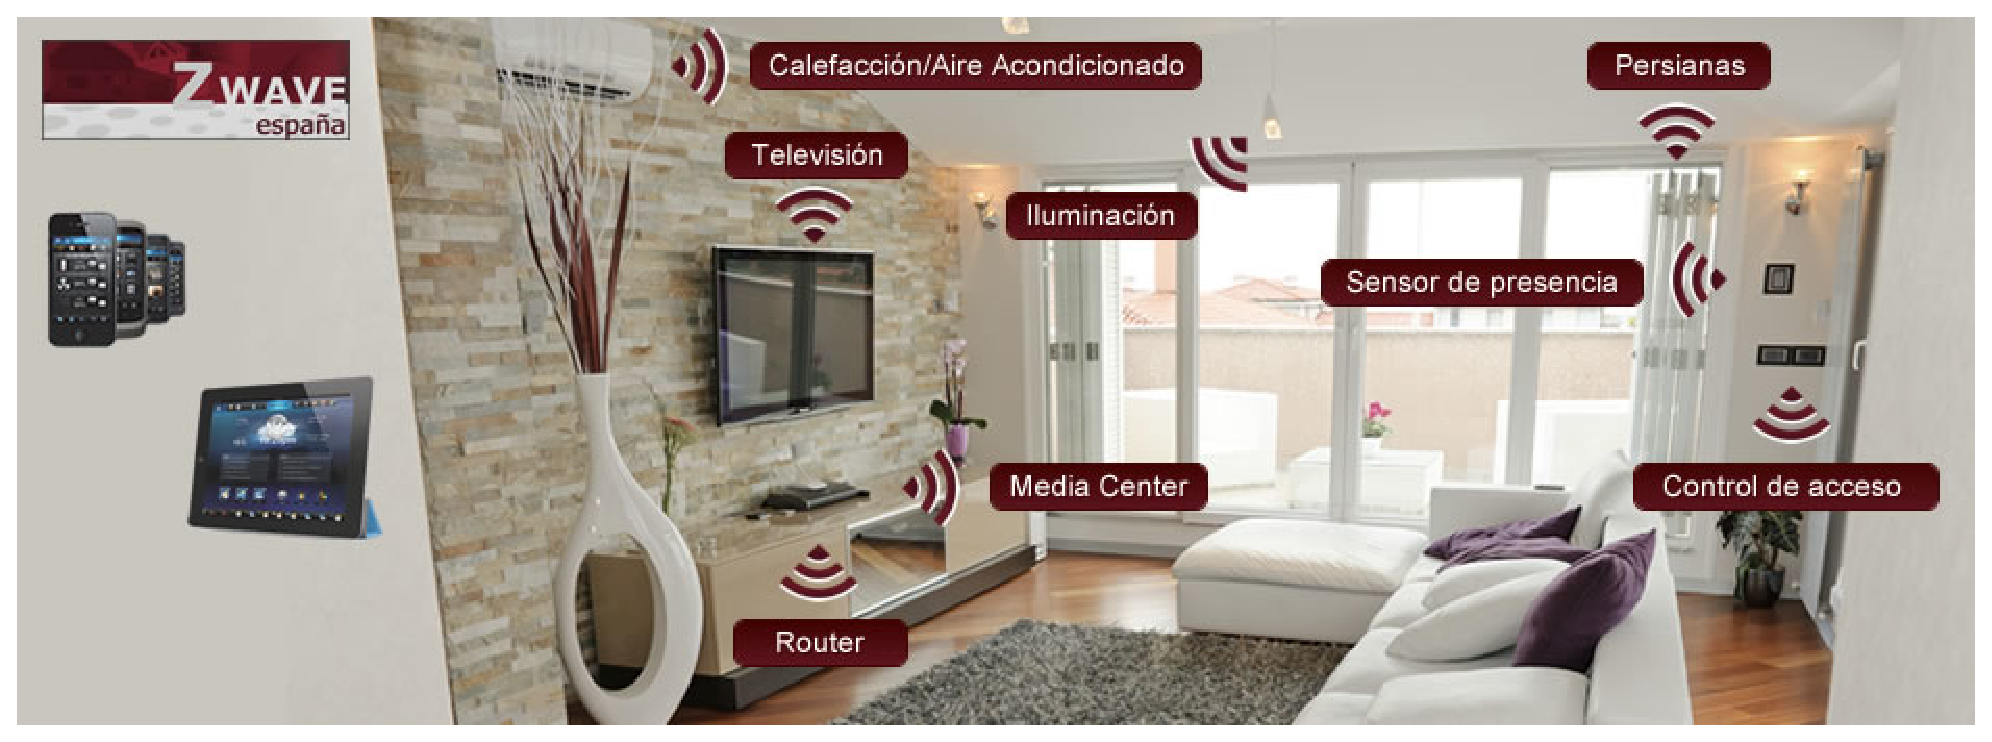
\includegraphics[keepaspectratio,width=0.9\textwidth]{z-wave.eps}
    \caption{Z-Wave}\label{fig:z-wave}
\end{figure}

La integración de \emph{Arduino} con el estándar \emph{Z-Wave} no es sencillo. Es posible encontrar módulos wireless que con sompatibles con la frecuencia que emiten los componentes \emph{Z-Wave} pero hay que implementarse todo el protocolo \emph{Z-Wave} de comunicación, lo cual no es sencillo.

Además, si se optara por realizar esta integraciía, sería necesario contar un servidor \emph{Z-Wave} para realizar la comunicación. Y los productos de \emph{Z-Wave} tienen un precio bastante elevado, por lo que el coste final del proyecto ascendería, lo cual no cumple con uno de los objetivos de realizar un componente barato.